\documentclass[aspectratio=169,utf8,t]{beamer}

% Idioma e Codificacao
\usepackage[brazilian]{babel}
\usepackage{booktabs}
\usepackage{array}
\usepackage{listings}
\usepackage{amsmath}
\usepackage{amssymb}
\usepackage{graphicx}

% Carrega o Tema Modelo dos Scouts (Widescreen 16:9, Nunito Sans)
\usetheme{scouts}

% Configuracao para Codigo-Fonte (Python / JSON / Bash)
\lstset{
    basicstyle=\ttfamily\scriptsize,
    keywordstyle=\bfseries\color{ScoutNavy},
    stringstyle=\color{ScoutGreen},
    commentstyle=\itshape\color{gray},
    backgroundcolor=\color{black!3},
    frame=single,
    rulecolor=\color{black!15},
    breaklines=true,
    showstringspaces=false,
    tabsize=2
}

% Metadados Institucionais
\author{Prof. Me. Reginaldo Fernandes}
\institute{Instituto Federal do Ceará -- Campus Tauá \\ Tecnologia em Análise e Desenvolvimento de Sistemas}
\title{Bancos de Dados Não-Relacionais}
\subtitle{Aula 03 (Sábado Letivo): Prática de MongoDB \& Redis (CLI, GUI e Python)}
\date{10 de Outubro de 2026}

\begin{document}

% ------------------------------------------------------------------------------
% Capa da Apresentacao
% ------------------------------------------------------------------------------
\changecolours[inverse]{ScoutGreen}
\frame[plain]{\titlepage}

% ------------------------------------------------------------------------------
% Sumario Executivo da Aula
% ------------------------------------------------------------------------------
\changecolours{ScoutGreen}
\begin{frame}{Roteiro de Atividades -- Sábado Letivo (Não-Presencial)}
  \vspace{0.4cm}
  \tableofcontents
\end{frame}

% ------------------------------------------------------------------------------
% Modulos da Aula
% ------------------------------------------------------------------------------
% ==============================================================================
% SEÇÃO 1: AMBIENTE DE ESTUDO REMOTO E ARQUITETURA HÍBRIDA
% ==============================================================================
\changecolours{ScoutNavy}
\section{Ambiente Remoto e Arquitetura Híbrida}

\begin{frame}{Contexto Pedagógico: Sábado Letivo Autônomo}
  \begin{columns}[T]
    \begin{column}{0.50\textwidth}
      \begin{block}{Objetivo Central da Prática}
        {\footnotesize Dominar CRUD no MongoDB e no Redis, unindo-os através do padrão \textbf{Cache-Aside}.}
      \end{block}
      \vspace{0.2cm}
      {\footnotesize
      \begin{itemize}
        \item \textbf{Nivelamento Prático:} Domínio direto via CLI e GUIs.
        \item \textbf{Arquitetura:} Persistência durável vs RAM de baixa latência.
      \end{itemize}
      }
    \end{column}

    \begin{column}{0.48\textwidth}
      \begin{exampleblock}{Duas Trilhas de Execução}
        {\footnotesize
        \textbf{1. Nuvem + Desktop GUI:}\\
        MongoDB Atlas Free + Compass e Redis Cloud + Redis Insight.\\[6pt]
        \textbf{2. Containers Locais (Docker):}\\
        Provisionamento com comando único:\\[3pt]
        \centering\texttt{docker compose up -d}
        }
      \end{exampleblock}
    \end{column}
  \end{columns}
\end{frame}

\begin{frame}{Opção 1: Setup em Nuvem com GUIs Oficiais}
  \begin{columns}[T]
    \begin{column}{0.50\textwidth}
      \textbf{MongoDB Atlas \& Compass}
      {\footnotesize
      \begin{enumerate}
        \item Criar conta gratuita no \textbf{MongoDB Atlas}.
        \item Criar cluster compartilhado \textbf{M0} (512 MB).
        \item Em \textit{Database Access}, criar usuário/senha.
        \item Em \textit{Network Access}, liberar seu IP (\texttt{0.0.0.0/0}).
        \item Baixar o \textbf{MongoDB Compass} e conectar via string SRV (\texttt{mongodb+srv://...}).
      \end{enumerate}
      }
    \end{column}

    \begin{column}{0.50\textwidth}
      \textbf{Redis Cloud \& Redis Insight}
      {\footnotesize
      \begin{enumerate}
        \item Baixar o \textbf{Redis Insight} (\url{redis.io/insight}).
        \item Conectar em instância local (\texttt{localhost:6379}) ou Redis Cloud gratuito (30 MB).
        \item Acessar navegador de chaves em árvore (\textit{Key Tree}) e terminal CLI integrado.
        \item Analisar estruturas e consumo de memória RAM.
      \end{enumerate}
      }
    \end{column}
  \end{columns}
\end{frame}

\begin{frame}{Opção 2: Setup Local via Docker Compose}
  \begin{columns}[T]
    \begin{column}{0.50\textwidth}
      \begin{exampleblock}{Comando Único de Inicialização}
        {\centering\small\texttt{docker compose up -d}\par}
      \end{exampleblock}
      \vspace{0.2cm}
      {\footnotesize
      \textbf{Serviços Subindo no Host:}
      \begin{itemize}
        \item \textbf{MongoDB 8.0} (\texttt{:27017}) + \textbf{Express} (\texttt{:8081})
        \item \textbf{Redis 7.4} (\texttt{:6379}) + \textbf{Insight} (\texttt{:5540})
      \end{itemize}
      }
    \end{column}

    \begin{column}{0.46\textwidth}
      \begin{block}{Vantagens do Ambiente Local}
        {\footnotesize
        \begin{itemize}
          \item Reprodutível em Linux, Windows e macOS.
          \item Volumes persistentes pré-configurados.
          \item Não polui o sistema operacional host.
          \item Para encerrar: \texttt{docker compose down}.
        \end{itemize}
        }
      \end{block}
    \end{column}
  \end{columns}
\end{frame}

\begin{frame}{Visão Arquitetural Híbrida: MongoDB + Redis}
  \centering
  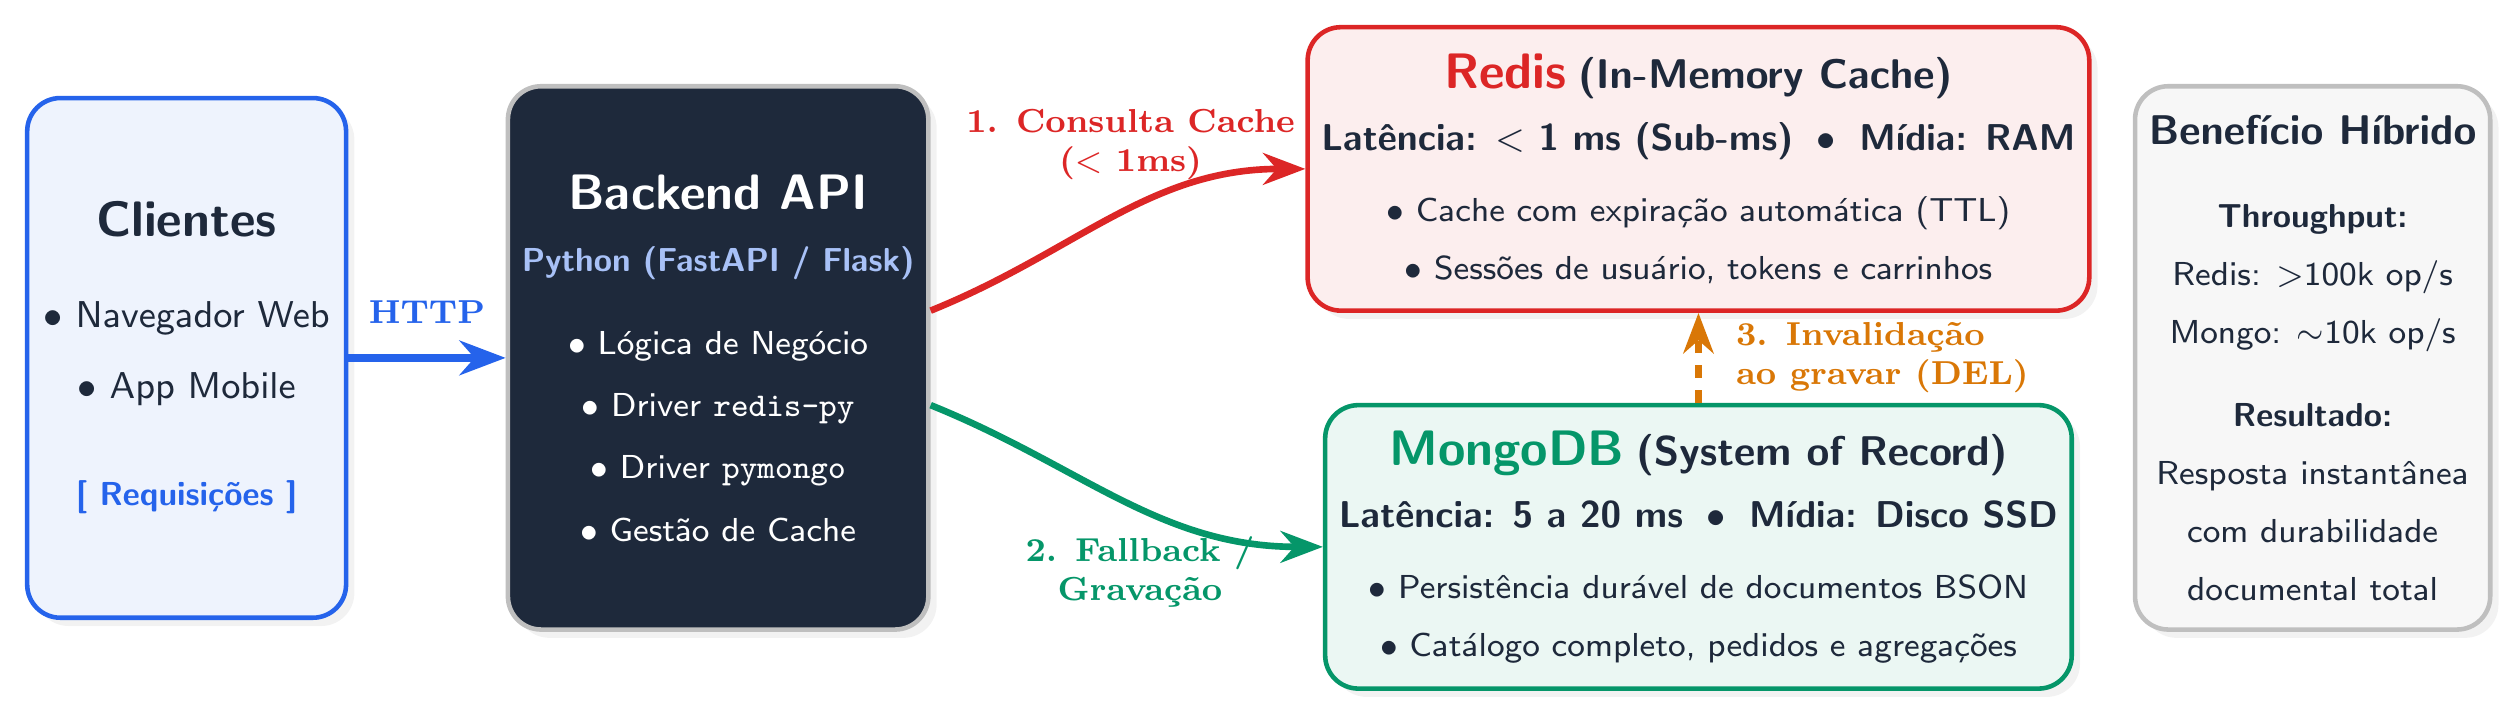
\includegraphics[width=0.98\textwidth,height=0.82\textheight,keepaspectratio]{figuras/fig_arquitetura_hibrida.png}
\end{frame}

% ==============================================================================
% SEÇÃO 2: PRÁTICA MONGODB DIRETO NO BANCO (SEM PYTHON)
% ==============================================================================
\changecolours{ScoutGreen}
\section{MongoDB Direto no Banco: CLI \& GUI}

\begin{frame}{Modelo Documental BSON no MongoDB Compass}
  \centering
  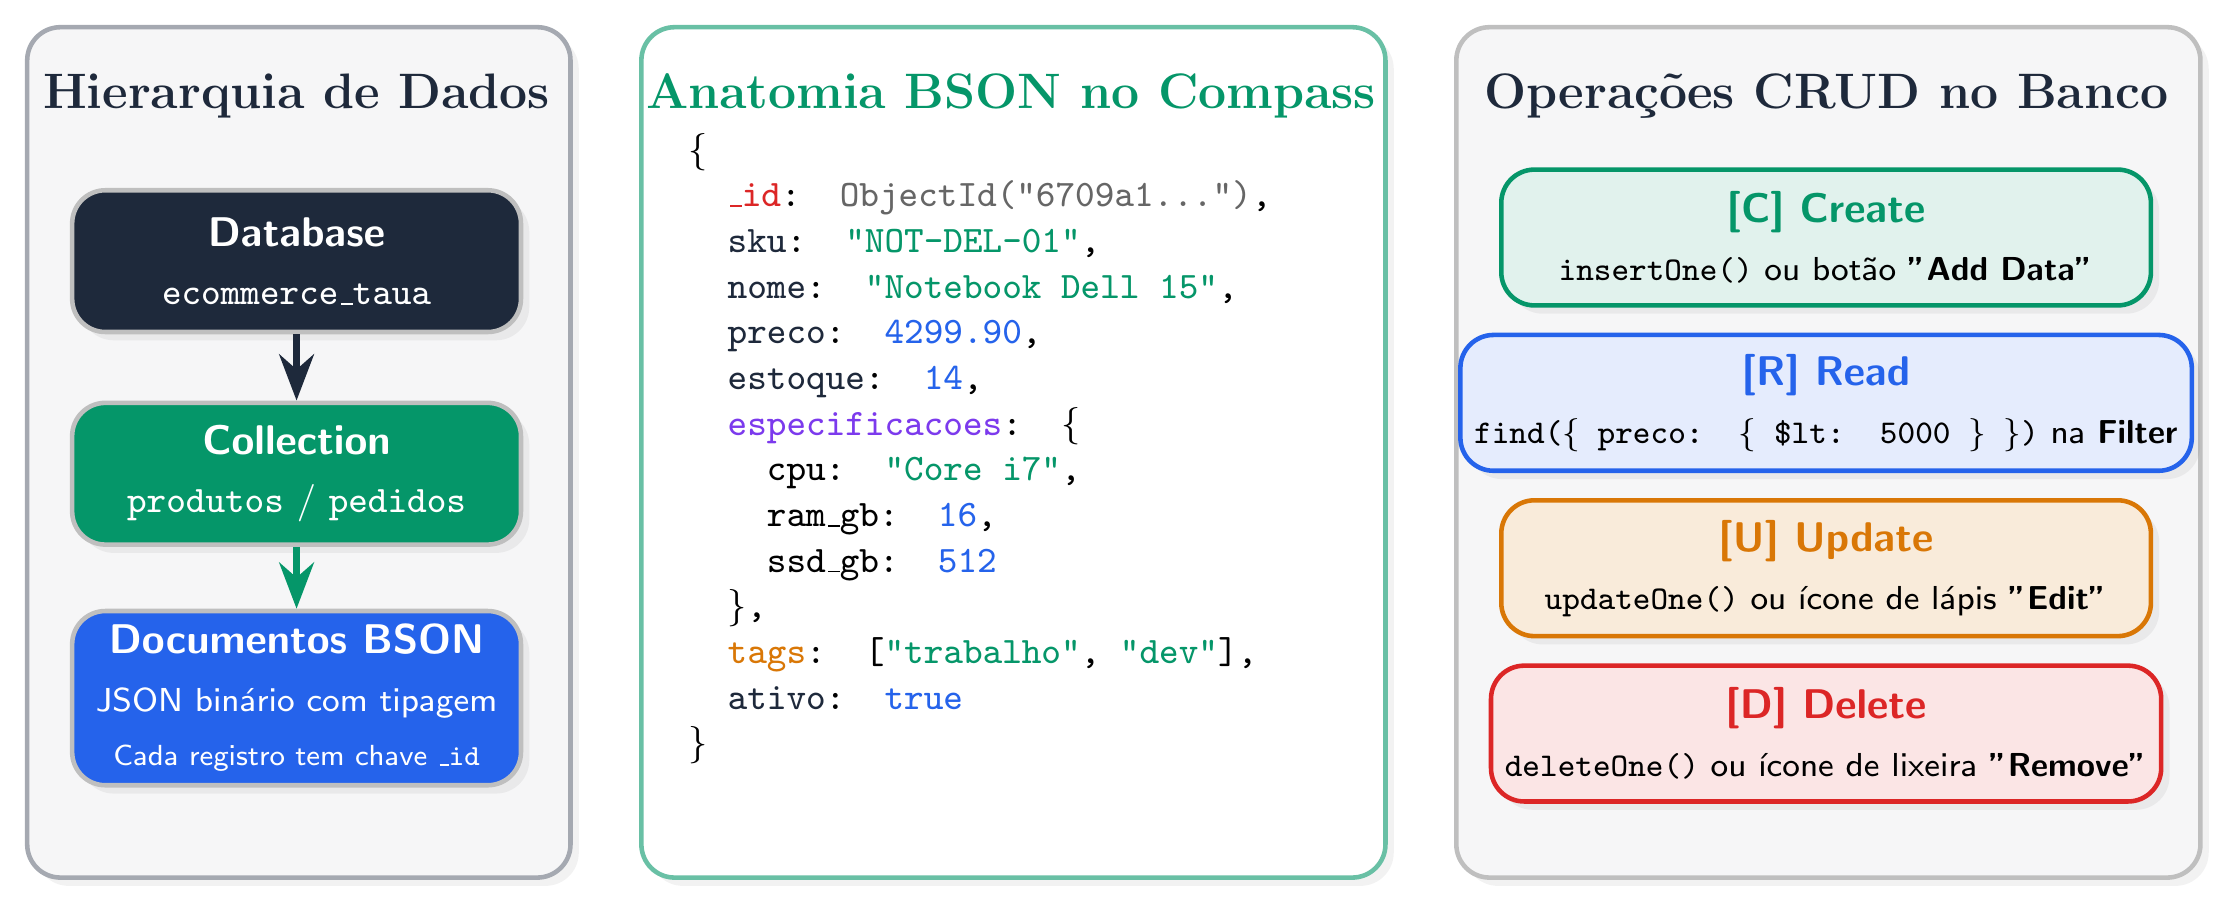
\includegraphics[width=0.98\textwidth,height=0.82\textheight,keepaspectratio]{figuras/fig_mongo_crud_compass.png}
\end{frame}

\begin{frame}{Operando no MongoDB Compass (Interface Gráfica)}
  \begin{columns}[T]
    \begin{column}{0.48\textwidth}
      \textbf{Passo a Passo Visual no Compass}
      {\footnotesize
      \begin{enumerate}
        \item Conectar em \texttt{localhost:27017} (ou Atlas).
        \item Criar banco \texttt{ecommerce\_taua} / \texttt{produtos}.
        \item Clicar em \textbf{Add Data} $\rightarrow$ \textbf{Insert Document}.
        \item Alternar para visualização \textbf{JSON} e colar.
        \item Clicar em \textbf{Insert} para persistir.
      \end{enumerate}
      }
    \end{column}

    \begin{column}{0.50\textwidth}
      \begin{block}{Consultas na Barra Filter}
        {\footnotesize
        \begin{itemize}
          \item \textbf{Filtro de Categoria:}\\
            {\scriptsize\texttt{\{ categoria: "Perifericos" \}}}
          \item \textbf{Filtro de Preço:}\\
            {\scriptsize\texttt{\{ preco: \{ \$lt: 1000 \} \}}}
          \item \textbf{Projeção} (\textit{Project}):\\
            {\scriptsize\texttt{\{ nome: 1, preco: 1, \_id: 0 \}}}
        \end{itemize}
        }
      \end{block}
    \end{column}
  \end{columns}
\end{frame}

\begin{frame}[fragile]{Terminal mongosh: Criação e Inserção Individual}
  \textbf{Seleção de Banco e Inserção com \texttt{insertOne}:}
\begin{lstlisting}[basicstyle=\ttfamily\scriptsize]
// 1. Criar e selecionar o banco de dados
use ecommerce_taua

// 2. Inserir documento individual rico com atributos aninhados
db.produtos.insertOne({
  sku: "NOT-DEL-01",
  nome: "Notebook Dell Inspiron 15",
  categoria: "Informatica",
  preco: 4299.90,
  estoque: 14,
  especificacoes: { processador: "Core i7", ram_gb: 16, ssd_gb: 512 },
  tags: ["trabalho", "desenvolvimento", "bivolt"],
  ativo: true
})
\end{lstlisting}
\end{frame}

\begin{frame}[fragile]{Terminal mongosh: Inserção em Lote (insertMany)}
  \textbf{Inserção Múltipla com Eficiência de Rede (\textit{Bulk Insert}):}
\begin{lstlisting}[basicstyle=\ttfamily\scriptsize]
db.produtos.insertMany([
  { sku: "MOU-LOG-02", nome: "Mouse Logitech MX",
    categoria: "Perifericos", preco: 589.00, estoque: 30 },
  { sku: "TEC-MEC-03", nome: "Teclado Keychron K2",
    categoria: "Perifericos", preco: 699.50, estoque: 20 },
  { sku: "MON-DEL-04", nome: "Monitor Dell 27 4K",
    categoria: "Monitores", preco: 2890.00, estoque: 8 }
])
\end{lstlisting}
  {\footnotesize
  \begin{itemize}
    \item Reduz \textit{round-trips} de rede agrupando registros em pacote único.
    \item Retorna um array com os \texttt{insertedIds} gerados automaticamente.
  \end{itemize}
  }
\end{frame}

\begin{frame}[fragile]{Terminal mongosh: Consultas Básicas e Projeção}
  \textbf{Filtros de Comparação e Seleção de Campos:}
\begin{lstlisting}[basicstyle=\ttfamily\scriptsize]
// 1. Buscar todos os documentos projetando apenas sku, nome e preco
db.produtos.find(
  {},
  { _id: 0, sku: 1, nome: 1, preco: 1 }
)

// 2. Filtrar produtos por categoria e preco menor que R$ 650 ($lt)
db.produtos.find({
  categoria: "Perifericos",
  preco: { $lt: 650.00 }
})
\end{lstlisting}
\end{frame}

\begin{frame}[fragile]{Terminal mongosh: Consultas em Arrays e Subdocumentos}
  \textbf{Busca em Estruturas Aninhadas (Dot-Notation):}
\begin{lstlisting}[basicstyle=\ttfamily\scriptsize]
// 1. Busca exata dentro de array de tags
db.produtos.find({ tags: "desenvolvimento" })

// 2. Consulta em objeto aninhado usando notacao de ponto
db.produtos.find({ "especificacoes.ram_gb": { $gte: 16 } })

// 3. Ordenacao decrescente por preco e limite
db.produtos.find().sort({ preco: -1 }).limit(3)
\end{lstlisting}
\end{frame}

\begin{frame}[fragile]{Terminal mongosh: Atualizações Atômicas e Remoção}
  \begin{columns}[T]
    \begin{column}{0.50\textwidth}
      \textbf{Modificações (\$set, \$inc, \$push)}
\begin{lstlisting}[basicstyle=\ttfamily\tiny]
// Atualizar preco e adicionar tag
db.produtos.updateOne(
  { sku: "NOT-DEL-01" },
  {
    $set: { preco: 3899.00 },
    $push: { tags: "liquidacao" }
  }
)

// Incrementar estoque de forma atomica
db.produtos.updateOne(
  { sku: "MOU-LOG-02" },
  { $inc: { estoque: 5 } }
)
\end{lstlisting}
    \end{column}

    \begin{column}{0.50\textwidth}
      \textbf{Deleção e Índices}
\begin{lstlisting}[basicstyle=\ttfamily\tiny]
// Remover documento individual
db.produtos.deleteOne({
  sku: "CAB-USBC-05"
})

// Remover produtos inativos
db.produtos.deleteMany({
  ativo: false
})

// Criar indice para busca veloz
db.produtos.createIndex({
  categoria: 1
})
\end{lstlisting}
    \end{column}
  \end{columns}
\end{frame}

% ==============================================================================
% SEÇÃO 3: PRÁTICA REDIS DIRETO NO BANCO (SEM PYTHON)
% ==============================================================================
\changecolours{ScoutRed}
\section{Redis Direto no Banco: CLI \& Redis Insight}

\begin{frame}{As 5 Estruturas de Dados Fundamentais do Redis}
  \centering
  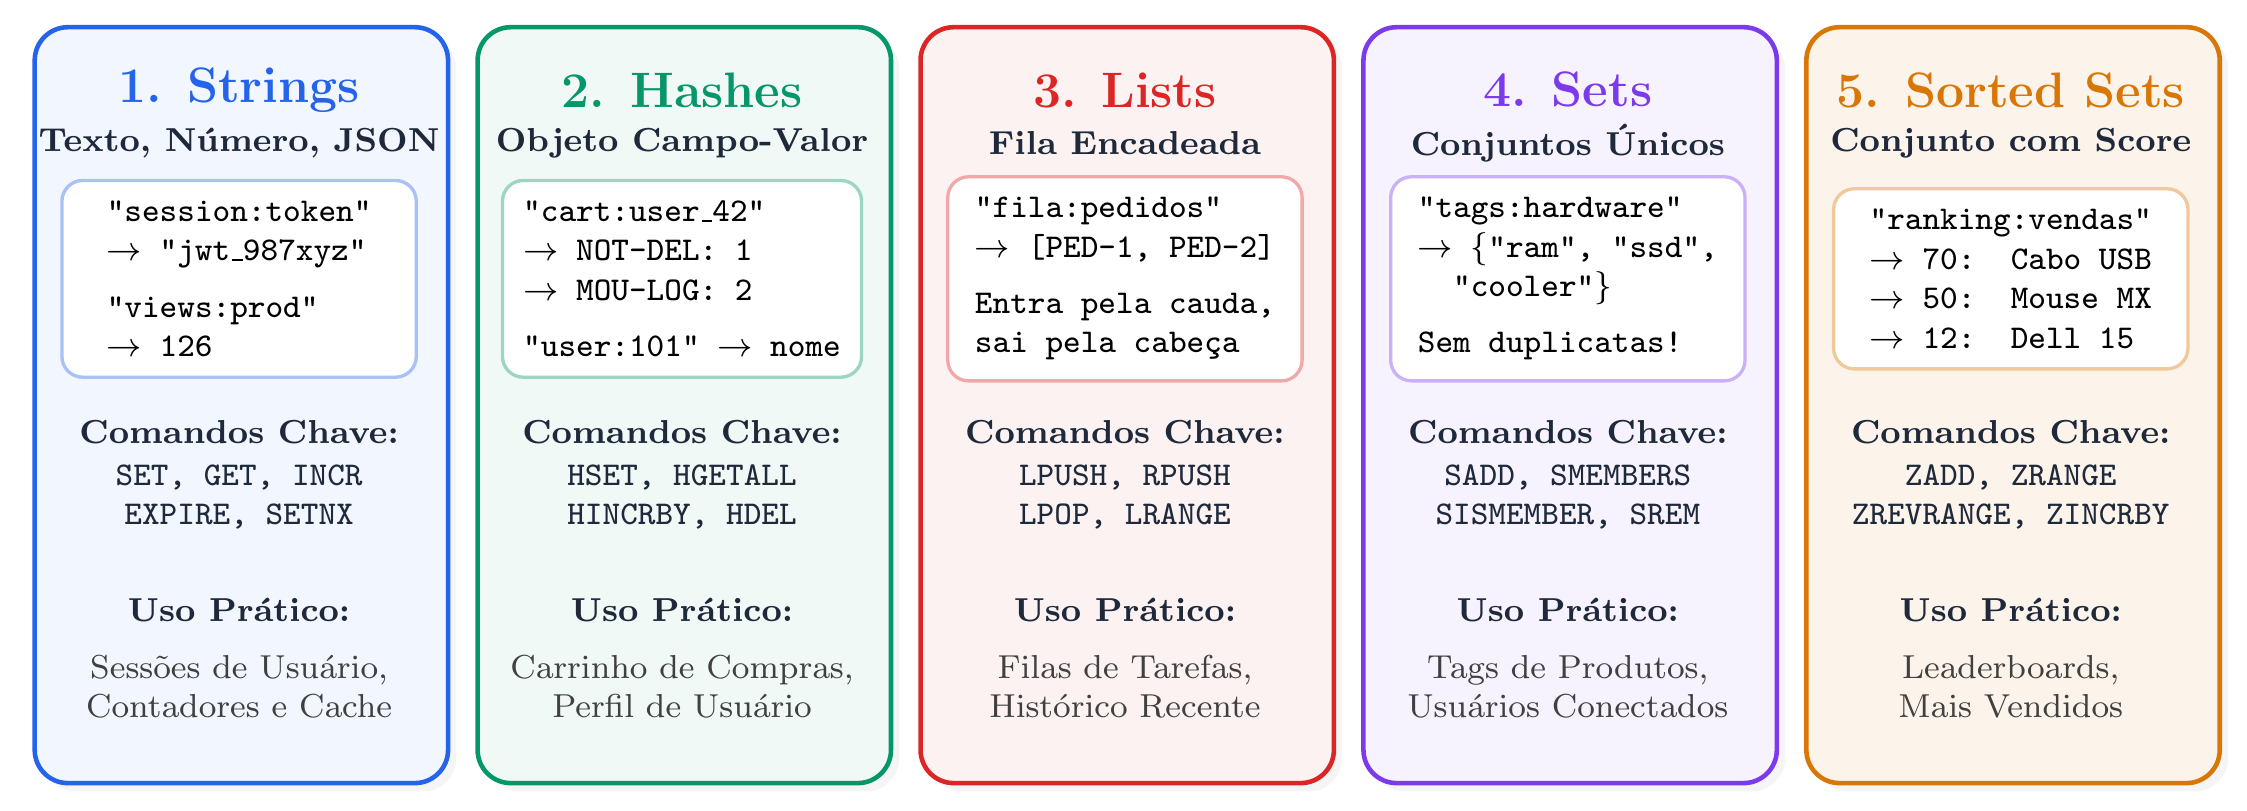
\includegraphics[width=0.98\textwidth,height=0.82\textheight,keepaspectratio]{figuras/fig_redis_estruturas.png}
\end{frame}

\begin{frame}{Operando com Redis Insight (Interface Gráfica)}
  \begin{columns}[T]
    \begin{column}{0.54\textwidth}
      \textbf{Recursos Visuais do Redis Insight}
      {\footnotesize
      \begin{enumerate}
        \item \textbf{Key Tree:} organiza chaves hierárquicas separadas por \texttt{:}.
        \item \textbf{Editor Visual:} inspeciona e edita Hashes, Listas e Sets em tempo real.
        \item \textbf{Memory Profiler:} analisa consumo de memória RAM por padrão de chave.
        \item \textbf{CLI Embutido:} terminal interativo acessível no rodapé.
      \end{enumerate}
      }
    \end{column}

    \begin{column}{0.44\textwidth}
      \begin{block}{Padrão de Nomes de Chaves}
        {\footnotesize
        Convenções recomendadas:
        \begin{itemize}
          \item \texttt{entidade:id}\\[1pt]
            {\scriptsize Ex: \texttt{user:101}}
          \item \texttt{entidade:id:subtipo}\\[1pt]
            {\scriptsize Ex: \texttt{cart:user:42}}
          \item \texttt{servico:escopo:chave}\\[1pt]
            {\scriptsize Ex: \texttt{cache:prod:01}}
        \end{itemize}
        }
      \end{block}
    \end{column}
  \end{columns}
\end{frame}

\begin{frame}[fragile]{Terminal redis-cli: Strings, TTL e Contadores}
  \textbf{Operações Chave-Valor Básicas e Expiração Automática:}
\begin{lstlisting}[basicstyle=\ttfamily\scriptsize]
// 1. Sessao temporaria com TTL de 120s
SET session:ads_user_42 "token_jwt_987" EX 120
GET session:ads_user_42       // Retorna o valor
TTL session:ads_user_42       // Retorna segundos restantes

// 2. Contador atomico de acessos
INCR views:produto:NOT-DEL-01
INCRBY views:produto:NOT-DEL-01 25

// 3. Trava distribuida atomica (Lock idempotente)
SET lock:pedido:9001 "worker_1" NX EX 30
\end{lstlisting}
\end{frame}

\begin{frame}[fragile]{Terminal redis-cli: Hashes e Carrinho de Compras}
  \textbf{Modelagem de Objetos e Carrinhos com Hashes:}
\begin{lstlisting}[basicstyle=\ttfamily\scriptsize]
// 1. Criar entidade com multiplos campos
HSET user:101 nome "Reginaldo Fernandes" campus "Taua" nivel "Docente"

// 2. Consultar campo individual e o hash completo
HGET user:101 nome
HGETALL user:101

// 3. Modelagem de Carrinho de Compras (SKU -> Quantidade)
HSET cart:session_taua_77 "NOT-DEL-01" 1 "MOU-LOG-02" 2

// 4. Incrementar item de forma atomica
HINCRBY cart:session_taua_77 "MOU-LOG-02" 1
\end{lstlisting}
\end{frame}

\begin{frame}[fragile]{Terminal redis-cli: Listas, Conjuntos e Rankings}
  \begin{columns}[T]
    \begin{column}{0.50\textwidth}
      \textbf{Filas FIFO com Lists}
\begin{lstlisting}[basicstyle=\ttfamily\tiny]
// Produtor enfileira na cauda
RPUSH fila:pedidos "PED-1" "PED-2"

// Consumidor retira da cabeca
LPOP fila:pedidos

// Consultar fila sem remover
LRANGE fila:pedidos 0 -1
\end{lstlisting}
    \end{column}

    \begin{column}{0.50\textwidth}
      \textbf{Rankings com Sorted Sets}
\begin{lstlisting}[basicstyle=\ttfamily\tiny]
// Adicionar score de vendas
ZADD ranking 45 "MOU-LOG-02"
ZADD ranking 12 "NOT-DEL-01"
ZADD ranking 70 "CAB-USBC-05"

// Top 3 mais vendidos (decrescente)
ZREVRANGE ranking 0 2 WITHSCORES
\end{lstlisting}
    \end{column}
  \end{columns}
\end{frame}

% ==============================================================================
% SEÇÃO 4: INTEGRAÇÃO COMPLEMENTAR COM PYTHON (PADRÃO CACHE-ASIDE)
% ==============================================================================
\changecolours{ScoutBlue}
\section{Integração Complementar com Python: Cache-Aside}

\begin{frame}{O Padrão Arquitetural Cache-Aside (Lazy Loading)}
  \centering
  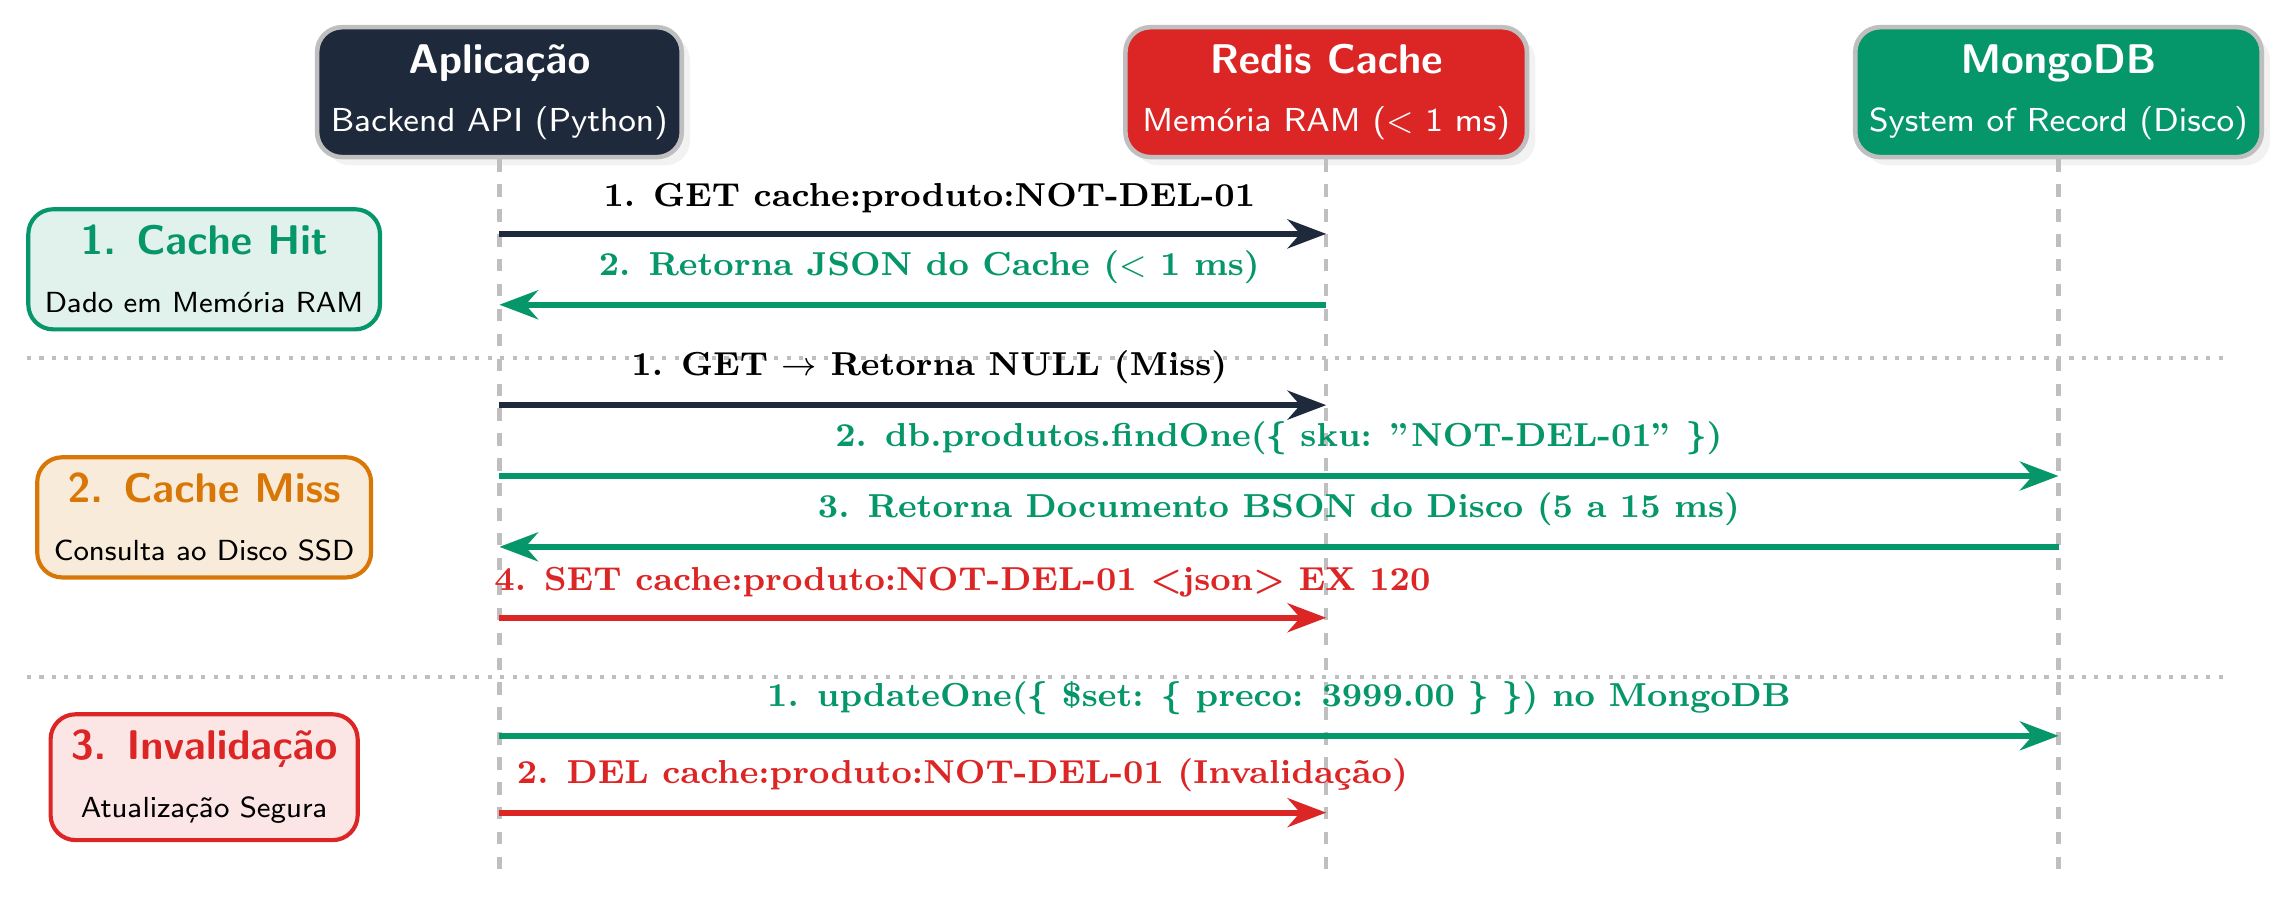
\includegraphics[width=0.98\textwidth,height=0.82\textheight,keepaspectratio]{figuras/fig_cache_aside_pattern.png}
\end{frame}

\begin{frame}[fragile]{Cache-Aside em Python: Verificação e Cache Hit}
  \textbf{Fluxo de Consulta em Memória RAM (Sub-milissegundo):}
\begin{lstlisting}[basicstyle=\ttfamily\scriptsize]
def obter_produto(sku: str, mongo_col, redis_cli, ttl=120):
    cache_key = f"cache:produto:{sku}"
    
    # 1. Tenta recuperar da memoria RAM (Redis)
    dado_cache = redis_cli.get(cache_key)
    if dado_cache:
        return json.loads(dado_cache), "CACHE_HIT"
\end{lstlisting}
  {\footnotesize
  \begin{itemize}
    \item \textbf{Cache Hit:} Resposta imediata da RAM ($< 1$ ms) sem sobrecarregar o MongoDB.
  \end{itemize}
  }
\end{frame}

\begin{frame}[fragile]{Cache-Aside em Python: Cache Miss e População}
  \textbf{Fallback no MongoDB e Armazenamento com TTL:}
\begin{lstlisting}[basicstyle=\ttfamily\scriptsize]
    # 2. CACHE MISS: Busca na fonte da verdade (MongoDB)
    produto_db = mongo_col.find_one({"sku": sku}, {"_id": 0})
    if not produto_db:
        return None, "NOT_FOUND"
        
    # 3. Popula o cache no Redis com tempo de vida definido (TTL)
    redis_cli.set(cache_key, json.dumps(produto_db), ex=ttl)
    return produto_db, "CACHE_MISS"
\end{lstlisting}
  {\footnotesize
  \begin{itemize}
    \item \textbf{Lazy Loading Idempotente:} O cache só é abastecido sob demanda, otimizando a memória RAM.
  \end{itemize}
  }
\end{frame}

\begin{frame}[fragile]{Invalidação de Cache e Prevenção de Dados Obsoletos}
  \begin{columns}[T]
    \begin{column}{0.52\textwidth}
      \textbf{Atualização com Invalidação}
\begin{lstlisting}[basicstyle=\ttfamily\scriptsize]
def atualizar_preco(sku, preco, col, r):
  # 1. Atualiza MongoDB
  col.update_one(
    {"sku": sku},
    {"$set": {"preco": preco}}
  )
  # 2. Invalida no Redis
  r.delete(f"cache:prod:{sku}")
\end{lstlisting}
    \end{column}

    \begin{column}{0.46\textwidth}
      \begin{block}{O Risco de Stale Read}
        {\footnotesize
        Sem invalidação ativa imediata:
        \begin{itemize}
          \item Usuários visualizam dados defasados até o TTL expirar.
          \item O comando \texttt{DEL} força o próximo acesso a buscar o valor atualizado na fonte oficial.
        \end{itemize}
        }
      \end{block}
    \end{column}
  \end{columns}
\end{frame}

\begin{frame}{Resultados Empíricos: Benchmarking de Latência}
  \centering
  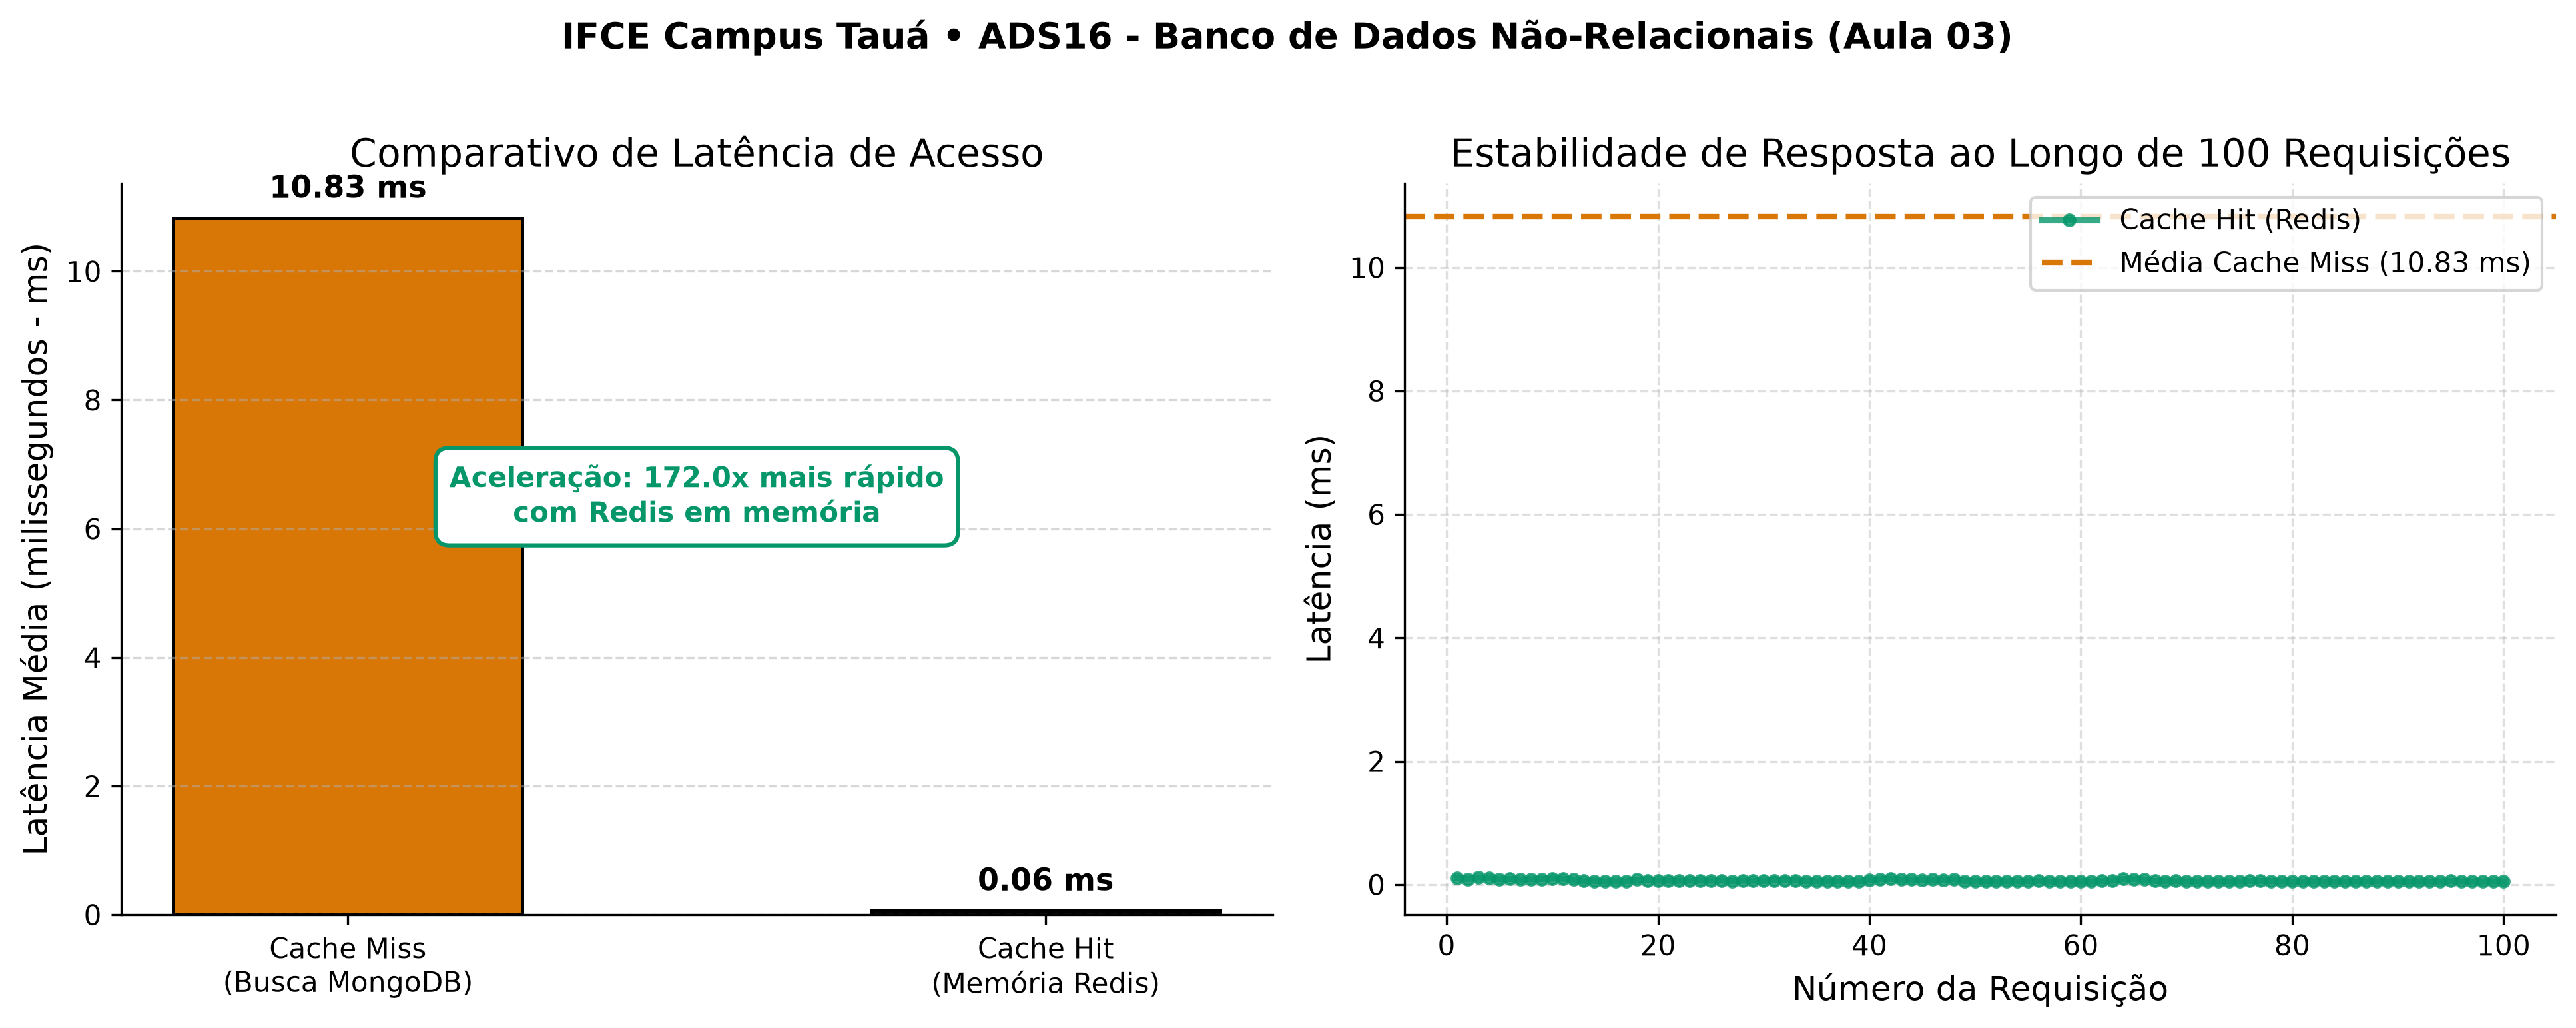
\includegraphics[width=0.98\textwidth,height=0.82\textheight,keepaspectratio]{figuras/grafico_latencia_cache.png}
\end{frame}

% ==============================================================================
% SEÇÃO 5: ROTEIRO DA LISTA DE EXERCÍCIOS DE FIXAÇÃO
% ==============================================================================
\changecolours{ScoutPurple}
\section{Roteiro da Lista de Exercícios Práticos}

\begin{frame}{Estrutura da Lista de Exercícios (Entrega Sábado Letivo)}
  \begin{columns}[T]
    \begin{column}{0.48\textwidth}
      \textbf{Bloco 1: MongoDB (Sem Python)}
      {\footnotesize
      \begin{itemize}
        \item \textbf{Ex 1 (Modelagem):} Coleção com 5 documentos ricos no \texttt{mongosh}.
        \item \textbf{Ex 2 (Consultas):} 3 buscas com operadores \texttt{\$gt}, \texttt{\$in} e dot-notation.
        \item \textbf{Ex 3 (GUI Compass):} Criar índice e analisar na aba \textit{Explain Plan}.
      \end{itemize}
      }
    \end{column}

    \begin{column}{0.48\textwidth}
      \textbf{Bloco 2: Redis (Sem Python)}
      {\footnotesize
      \begin{itemize}
        \item \textbf{Ex 4 (Sessão \& TTL):} 3 tokens com TTL de 90s no \texttt{redis-cli}.
        \item \textbf{Ex 5 (Hashes - Carrinho):} Carrinho com \texttt{HSET} e \texttt{HINCRBY}.
        \item \textbf{Ex 6 (Redis Insight):} Print da árvore de chaves (\textit{Key Tree}) e análise de RAM.
      \end{itemize}
      }
    \end{column}
  \end{columns}
\end{frame}

\begin{frame}{Bloco 3: Integração e Diretrizes de Submissão}
  \begin{columns}[T]
    \begin{column}{0.50\textwidth}
      \textbf{Bloco 3: Integração com Python}
      {\footnotesize
      \begin{itemize}
        \item \textbf{Ex 7 (Cache-Aside):} Consulta no MongoDB com cache no Redis (TTL de 45s).
        \item \textbf{Ex 8 (Invalidação):} Atualização com remoção imediata (\texttt{DEL}) do Redis.
      \end{itemize}
      }

      \begin{block}{Critério de Avaliação}
        {\footnotesize Autonomia, prints das GUIs e código documentado.}
      \end{block}
    \end{column}

    \begin{column}{0.48\textwidth}
      \begin{exampleblock}{Instruções de Entrega}
        {\footnotesize
        \begin{itemize}
          \item \textbf{Prazo:} Até a sexta-feira anterior à Aula 04.
          \item \textbf{Formato:} PDF com comandos e prints ou repositório GitHub.
          \item \textbf{Envio:} SIGAA / Classroom.
        \end{itemize}
        }
      \end{exampleblock}
    \end{column}
  \end{columns}
\end{frame}


% ------------------------------------------------------------------------------
% Encerramento
% ------------------------------------------------------------------------------
\changecolours[inverse]{ScoutGreen}
\begin{frame}[plain]
  \vspace{2cm}
  \centering
  {\Huge \textbf{Dúvidas \& Suporte Remoto}}\par
  \vspace{0.8cm}
  {\large IFCE Campus Tauá -- ADS16 (Sábado Letivo)}\par
  \vspace{0.3cm}
  {\small Atendimento via Fórum SIGAA / GitHub Classroom}\par
  \vspace{0.2cm}
  {\small reginaldo.fernandes@ifce.edu.br}
\end{frame}

\end{document}
